\section{Namespaces as Document Clusters} \label{sec:namespaces-top}


In this chapter, we discuss how the process of namespace discovery
can be automated.

First, in section~\ref{sec:namespaces} we describe identifier namespaces and
we compare the namespace discovery with cluster analysis techniques
applied to textual data and see how clustering algorithms can be
useful. Next, in section~\ref{sec:vsm}
we review the Vector Space Model (VSM): the traditional way of
representing a collection of documents as vectors, and then in
section~\ref{sec:ism} we introduce the Identifier VSM - which
is a way to represent identifier-definition relations in the
vector space. Finally we go over common similarity and distance
functions that are useful for document clustering in
section~\ref{sec:similarity-distance} and discuss how similarity
search can be made faster by using inverted index~\ref{sec:index}.





\subsection{Vector Space Model} \label{sec:vsm}

Vector Space Model is a statistical model for representing documents
in some vector space. It is an Information Retrieval
model \cite{manning2008introduction}, but it is also used for various
Text Mining tasks such as Document Classification \cite{sebastiani2002machine}
and Document Clustering \cite{oikonomakou2005review} \cite{aggarwal2012survey}.

The process of transforming a text to its vector representation is
called ``vectorization''. But before documents can be
vectorized they are preprocessed. The preprocessing usually consists of the
following steps:

\begin{itemize}
\itemsep1pt\parskip0pt\parsep0pt
  \item tokenization: extracting individual words from the text;
  \item stop words removal: removes functional words that have no discriminative power;
  \item word normalization (includes stemming or lemmatization): reduces words to some common form;
\end{itemize}

There are two assumptions made about the data:

\begin{itemize}
\itemsep1pt\parskip0pt\parsep0pt
  \item \emph{Bag of Words assumption}: the order of words is not important,
     only word counts;
  \item \emph{Independence assumption}: we treat all words as independent.
\end{itemize}

% Bag of Words = unordered list of terms
% good enough for topic similarity

Both assumptions are quite strong, but nonetheless this method often
gives good results.


Document-Term Matrix - representation of a document for text analysis
each row of the matrix - is a ''document vector''
each component of the document vectors is a concept, a key word, or a term, but usually it's terms
documents don't contain many distinct words, so the matrix is sparse


Notation:
let $\mathcal D = \{d_1, \ ... \ , d_n \}$ be a set of $m$ documents
and let $\mathcal V = \{t_1, \ ... \ , t_m \}$ be a set of $n$ terms (the vocabulary).
Each document is set of weighed terms $d_i = \{ w_1, \ ... \ , w_m \}$
where $w_j$ is the weight of term $t_j$.

There are following term weighting schemes \cite{manning2008introduction}:

\begin{itemize}
\itemsep1pt\parskip0pt\parsep0pt
  \item binary: 1 if a term is present, 0 otherwise
  \item term frequency (TF): number of occurrences of the term in a document
  \item document frequency (DF): number of documents containing the term
  \item TF-IDF: combination of TF and inverse DF
\end{itemize}


\textbf{Term Frequency (TF)} weights terms by local frequency in the document.
That is, the term is weighed by how many times it occurs in the document.
We can define TF formally as
$$\text{tf}(t, d) = \big| \{ t' \in d  \ : \ t' = t \} \big|$$


\textbf{Sublinear TF}: sometimes the term is used too often in
a document and we want to reduce its influence compared to
other less frequent tokens. This can be done by applying
some sublinear transformation to TF, for instance, a squared root
$\sqrt{\text{tf}(w, d)}$ or a logarithm $\log \text{tf}(w, d)$.


\textbf{Document Frequency (DF)} weights terms by their global frequency
in the collection, which is the number of documents that contain the token.
Formally it can be defined as
$$\text{df}(t, \mathcal D) = \big| \{ d \in \mathcal D \ : \  t \in d \} \big|$$


\textbf{Inverse Document Frequency (IDF)}: more often we are interested
in domain specific words than in neutral words, and these domain specific
words tent to occur less frequently and they usually have more discriminative
power: that is, they are better in telling one document apart from another.
So IDF should give more weights to rare words rather than to frequent words.
Typically IDF is defined as follows:
$$\text{idf}(t, \mathcal D) = \log \cfrac{ |\mathcal D| }{\text{df}(t, \mathcal D)}$$



A good weighting system gives the best performance when it assigns
more weights to terms with high TF, but low DF \cite{salton1988term}.
This can be achieved by combining both TF and IDF
schemes. TF is good for getting high frequency words, but using
just TF is not enough if high frequency words are contained in
many documents, thus need a collection dependent factor that favors
terms that are contained in fewer documents: IDF.

Usually a sublinear TF is used to avoid the dominating effect of
words that occur too frequently. As the result, terms appearing
too rarely or too frequently are ranked low.

So, we can combine TF and IDF then my multiplying:
$$\text{tf-idf}(t, d \mid \mathcal D) = (1 + \log \text{tf}(t, d)) \cdot \log \cfrac{|\mathcal D|}{\text{df}(t, \mathcal D)}$$


\ \\

Once the weighting scheme is established, documents can be represented
by vectors $d_i = (w_1, \ ... \ w_m)$ where $w_j$ is the weight of term
$t_j$.

Then these vectors can be put together to form a matrix. Let $D$ be
a $m \times n$ matrix, where rows of $D$ are indexed by terms $t_i$,
columns of $D$ are indexed by documents $d_j$, and element $(D)_{ij}$
is a weight $w_i$ of term $t_i$ in document $d_j$. Then
such matrix $D$ is called a \emph{term-document matrix}.

Alternatively, $D$ can be $n \times m$ matrix with rows being indexed
by documents $d_j$ and columns - by terms $t_i$. Then such $D$ is called
\emph{document-term matrix}. Note that if $D$ is a term-document matrix,
then $D^T$ is a document-term matrix. In Information Retrieval
literature term-document matrices are used more often, than
document-term matrices, but in some applications, like Clustering,
it is more convenient to use document-term matrix.


Let us consider the column space of the term-document matrix $D$.
The column of $D$ are documents from the corpus $\mathcal D$,
so the column space of $D$ contains document vectors where
dimensions are terms $t_1,  t_2, \ ... \ , t_m$. This vector space is
called the \emph{Document VSM} (see fig.~\ref{fig:document-vsm}).

\begin{figure}[h]
\centering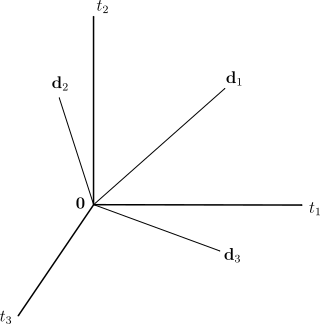
\includegraphics[width=0.6\textwidth]{document-vsm.png}
\caption{\textbf{TODO redraw in vector}}
\label{fig:document-vsm}
\end{figure}


\subsection{Identifier Space Model} \label{sec:ism}

The Vector Space Model gives a good foundation. In this work documents
are not represented by words they contain, but rather by identifiers they
have. Because  words and identifiers exhibit similar properties
(see section~\ref{sec:clusters-namespaces}) we can replace the
Term VSM by \emph{Identifier VSM}: a vector space where documents are represented as
vectors indexed by identifiers they contain.
Thus, the ``vocabulary'' of this space is $\text{id}_1, \ ... \ , \text{id}_k$, and
documents are represented as $d_j = (w_1, \ ... \ , w_k)$ where
$w_i$ is the weight of identifier $\text{id}_i$.

Then we can define an identifier-document matrix $D$ as $k \times n$
matrix where columns are documents and rows are identifers.

The Identifer VSM also suffers from the problems of polysemy
and synonymy (see section~\ref{sec:clusters-namespaces}). They
can be solved by extracting definitions for all the identifers
and incorporating these definitions into the Identifier VSM.

There are three ways of adding the definition information into
Identifier VSM:


\begin{itemize}
\itemsep1pt\parskip0pt\parsep0pt
  \item use only identifier information, and no not include the definitions;
  \item use ``weak'' identifier-definition association: include identifiers and
        definitions as separate dimensions;
  \item use ``strong'' association: append definition to identifier.
\end{itemize}

To illustrate how it is done, consider two relations ($\lambda$, ``regularization'')
and ($w$, ``weight vector'')


\begin{itemize}\itemsep1pt\parskip0pt\parsep0pt
  \item no definitions: dimension of the Identifier VSM are ($\lambda$, $w$)
  \item ``weak'' association:  dimensions are ($\lambda$, $w$, regularization, weight vector)
  \item ``strong'' association:  dimensions are ($\lambda$\_regularization, $w$\_weight vector)
\end{itemize}



\subsection{Similarity Measures and Distances} \label{sec:similarity-distance}

Once the documents are represented in some vector space, we need to
define how to compare these documents to each other. There are two
ways of doing this: using a similarity function that tells how similar
two objects are (the higher values, the more similar the objects),
or using a distance function, sometimes called ``dissimilarity function'',
which is the opposite of similarity (the higher the values, the less similar
the objects).

We will consider the following similarity and distance functions:


\begin{itemize}\itemsep1pt\parskip0pt\parsep0pt
  \item Euclidean distance
  \item Inner product (or dot product)
  \item Cosine similarity
  \item Jaccard coefficient
\end{itemize}


\subsubsection{Euclidean Distance} \ \\

The Euclidean distance function is the most commonly used distance
function in vector spaces. Euclidean distance corresponds to
the geometric distance between two data points in the vector space.
For example, if we have two points $\mathbf x$ and
$\mathbf z$, then the Euclidean distance is the
length of the line that connects these two points.
It is defined as
$$\| \mathbf x - \mathbf z \|^2 = (\mathbf x - \mathbf z)^T (\mathbf x - \mathbf z)  =\sum_i (x_i - z_i)^2$$

Euclidean distance is useful for low-dimensional data,
but it does not always work well in high dimensions, especially
with sparse vector such as document vectors \cite{ertoz2003finding}.



\subsubsection{Inner product} \ \\

The inner product between two vectors can be used as a similarity function:
the more similar two vectors are, the larger is their inner product.

Geometrically the inner product between two vectors $\mathbf x$ and $\mathbf z$
is defined as
$$\mathbf x^T \mathbf z = \|\mathbf x \| \, \| \mathbf z \| \, \cos \theta$$
where $\theta$ is the angle between vectors $\mathbf x$ and $\mathbf z$.
In Linear Algebra, however, the inner product
is defined as a sum of element-wise products of two vectors:
given two vectors $\mathbf x$ and $\mathbf z$, the inner product is
$\mathbf x^T \mathbf z = \sum_{i = 1}^n x_i \, z_i$ where $x_i$ and $z_i$
are $i$th elements of $\mathbf x$ and $\mathbf z$, respectively.
The geometric and algebraic definitions are equivalent \cite{huges2013calculus}.



\subsubsection{Cosine Similarity} \ \\


% However the magnitude of each individual vector still matters. If one
% document vector is particularly long compared to other vectors and it is not
% orthogonal to them (i.e. $\cos \theta \ne 0$), then it is likely to be
% one of the most similar vectors to others -- only because of its length.


Inner product is sensitive to the length of vectors, and thus
it may make sense to consider only the angle between them: 
the angle does not depend on the magnitude, but it is still
a very good indicator of vectors being similar or not.

The angle between two vectors can be calculated from the geometric
definition of inner product:
$\mathbf x^T \mathbf z = \|\mathbf x \| \, \| \mathbf z \| \, \cos \theta$.
By rearranging the terms we get
$$\cos \theta = \frac{\mathbf x^T \mathbf z}{\|\mathbf x \| \, \| \mathbf z \|} \ .$$ 

We do not need to the angle itself and can use the cosine directly
\cite{manning2008introduction}.
Thus can define \emph{cosine similarity} between two documents $\mathbf d_1$ and
$\mathbf d_2$ as
$$\text{cosine}(\mathbf d_1, \mathbf d_2) = \cfrac{\mathbf d_1^T \mathbf d_2}{\|\mathbf d_1 \| \, \| \mathbf d_2 \|} \ .$$
If the documents have unit lengths, then cosine similarity is the same as
dot product: $\text{cosine}(\mathbf d_1, \mathbf d_2) = \mathbf d_1^T \mathbf d_2$.

The cosine similarity can be converted to cosine distance.
The maximal possible cosine
is 1 for two identical documents. Therefore we can define \emph{cosine distance}
between two vectors $\mathbf d_1$ and $\mathbf d_2$ as
$d_c(\mathbf d_1, \mathbf d_2) = 1 - \text{cosine}(\mathbf d_1, \mathbf d_2)$. 
The cosine distance is not a proper metric \cite{korenius2007principal},
but it is nonetheless useful.

The cosine distance and the Euclidean distance are connected \cite{korenius2007principal}.
For two unit-normalized vectors $\mathbf d_1 = \mathbf d_1' / \| \mathbf d_1' \|$ and
$\mathbf d_2 = \mathbf d_1' / \| \mathbf d_1' \|$
the Euclidean distance between them is
$$\| \mathbf d_1 - \mathbf d_2 \|^2 = \| \mathbf d_1 \|^2 - 2 \, \mathbf d_1^T \mathbf d_2 + \| \mathbf d_2 \|^2 = 2 - 2 \, \mathbf d_1^T \mathbf d_2  .$$

Since the vectors are unit-normalized, we know that
$\text{cosine}(\mathbf d_1, \mathbf d_2) = \mathbf d_1^T \mathbf d_2$, so we have
$\| \mathbf d_1 - \mathbf d_2 \|^2 = 2 \, \big(1 - \text{cosine}(\mathbf d_1, \mathbf d_2)\big) = 2 \, d_c(\mathbf d_1, \mathbf d_2)$.


Thus we can use Euclidean distance on unit-normalized vectors
and interpret it as cosine distance.


\subsubsection{Jaccard Coefficient} \ \\

\textbf{Jaccard similarity, jaccard distance}


\subsection{Document Clustering Techniques} \label{sec:doc-clustering}

Cluster analysis is a set of techniques for
organizing collection of items into coherent groups.
In Text Mining clustering is often used for finding topics
in a collection of document.
In Information Retrieval clustering is used to assist the users and group
retrieved results into clusters.


There are several types of clustering algorithms:

\begin{itemize}
\itemsep1pt\parskip0pt\parsep0pt
  \item Hierarchical (Agglomerative and Divisive)
  \item Partitioning
  \item Density-based
  \item and others
\end{itemize}

In this chapter we will review some of the clustering techniques:
in section~\ref{sec:clustering-heierarchical} we will discuss
Agglomerative clustering. We discuss K-Means, a partitioning algorithms,
and its extensions in section~\ref{sec:kmeans-ext}.
Finally, a density-based algorithm DBSCAN is explained in
section~\ref{sec:dbscan} along with its extensions.


\subsection{Agglomerative clustering} \label{sec:clustering-heierarchical}

The general idea of agglomerative clustering algorithms is to start with
each document being its own cluster and iteratively merge clusters based
on best pair-wise cluster similarity.

Thus, a typical agglomerative clustering algorithms consists of the following steps:

\begin{enumerate}
\itemsep1pt\parskip0pt\parsep0pt
  \item let each document be a cluster on its own
  \item compute similarity between all pairs of clusters an store the
      results in a similarity matrix
  \item merge two most similar clusters
  \item update the similarity matrix
  \item repeat until everything belongs to the same cluster
\end{enumerate}

These algorithms differ only in the way they calculate
similarity between clusters.

It can be:

\begin{itemize}
\itemsep1pt\parskip0pt\parsep0pt
  \item \textbf{Single Linkage (SLINK)}: The clusters are merged based
on the closest pair. It can be very efficient, but it encourages
chaining behavior.

% similarity is usually not transitive:
%i.e. if $A$ is similar to $B$, and $B$ is similar to $C$, it doesn't mean that $A$ must be similar to $C$
% but single linkage encourages grouping through transitivity chains
% Sibson, Robin. "SLINK: an optimally efficient algorithm for the single-link cluster method." 1973.

  \item \textbf{Complete Linkage (CLINK)}: The clusters are merged
  based on the worst-case similarity - the similarity between the most
  distant objects on the clusters. It's very expensive computationally,
  but it avoids chaining altogether.

% Defays, Daniel. "An efficient algorithm for a complete link method." 1977.

  \item \textbf{Group-Average Linkage}: Similarity between clusters
  is calculated as average pair-wise similarity between all objects
  in the clusters, and the most similar clusters are merged.

  \item \textbf{Ward's Method}: The clusters to merge are chosen such that the within-cluster
  error (e.g. sum of squares) between each object and its centroid
  is minimized.

% El-Hamdouchi, Abdelmoula, and Peter Willett. "Hierarchic document classification using Ward's clustering method." 1986.

\end{itemize}


Among these algorithms only SLINK is computationally feasible
for large data sets, but it doesn't give good results compared to other
agglomerative clustering algorithms. Additionally, these algorithms
are not always good for document clustering because they tend to
make mistakes at early iterations that are impossible to correct
afterwards \cite{steinbach2000comparison}.



\subsection{$K$-Means} \label{sec:kmeans}

Unlike agglomerative clustering algorithms, K-Means is an iterative
algorithm, which means that it can correct the mistakes made
at earlier iterations.

Lloyd's algorithm  is the most popular way of implementing K-Means
\cite{xu2005survey}: given a desired number of clusters $k$,
it iteratively improves the Euclidean distance between each data
point and the centroid, closest to it.


Let $\mathcal D = \{  \mathbf d_1, \mathbf d_2, \ ... \ , \mathbf d_n \}$
be the document collection, where documents $\mathbf d_i$ are represented
is some document vector space $\mathbb R^m$ and $k$ is the desired
number of clusters. Then we define $k$ cluster centroids $\boldsymbol \mu_j$ that are
also in the same document vector space $\mathbb R^m$.
Additionally for each document $\mathbf d_i$ we maintain the assignment
variable $c_i \in \{ 1, 2, \ ... \ , k \}$, which specifies to what
cluster centroid $\boldsymbol \mu_1, \boldsymbol \mu_2, \ ... \ , \boldsymbol \mu_k$
the document $\mathbf d_i$ belongs.


The algorithms consists of three steps: (1) seed selection step,
where each $\boldsymbol \mu_j$ is randomly assigned some value,
(2) cluster assignment step, where we iterate over all document vectors
$\mathbf d_i$ and find its closest centroid, and (3)  move centroids step,
where the centroids are re-calculated. Steps (2) and (3) are repreated
until the algorithm converges. The pseudocode for $K$-Means is presented
in the listing~\ref{algo:k-means}.


\begin{algorithm}
\caption{Lloyd's algorithm for $K$-Means}
\label{algo:k-means}

\begin{algorithmic}[0]
  \Statex
  \Function{K-Means}{no. clusters $k$, documents $\mathcal D$}
    \For{$j \leftarrow 1 \ .. \ k$} \Comment{random seed selection}
      \Let{$\boldsymbol \mu_j$}{random $\mathbf d \in \mathcal D$}
    \EndFor

    \While{not converged}
      \For{each $\mathbf d_i \in \mathcal D$} \Comment{cluster assignment step}
        \Let{$c_i$}{$\operatorname{arg\, min}_j \| \mathbf d_i - \boldsymbol \mu_j \|^2$}
      \EndFor

      \For{$j \leftarrow 1 \ .. \ k$} \Comment{move centroids step}
        \Let{$\mathcal C_j$}{$\{\, \mathbf d_i \text{ s.t. } c_i = j \, \}$}
        \Let{$\boldsymbol \mu_j$}
            {$\cfrac{1}{| \mathcal C_j |} \sum_{\mathbf d_i \in \mathcal C_j} \mathbf d_i$}
      \EndFor
    \EndWhile

    \State \Return{$(c_1, c_2, \ ... \ , c_n)$}
  \EndFunction
\end{algorithmic}
\end{algorithm}

Usually, $K$-Means shows very good results for document clustering, and in
several studies it (or its variations) shows the best performance \cite{hall2012evaluating} \cite{steinbach2000comparison}.

However for large document collections Lloyd's classical $K$-Means takes a lot
of time to converge. The problem is caused by the fact that it goes through
the entire collection many times. Mini-Batch $K$-Means \cite{sculley2010web}
uses Mini-Batch Gradient Descent method, which is a different optimization technique
that converges faster. The pseudocode for Mini-Batch $K$-Means is presented
in listing~\ref{algo:minibatch-k-means}.

\begin{algorithm}
\caption{MiniBatch $K$-Means}
\label{algo:minibatch-k-means}

\begin{algorithmic}[0]
  \Statex
  \Function{MiniBatch-K-Means}{no. clusters $k$, no. iterations $t$, batch size $b$, documents $\mathcal D$}
    \For{$j \leftarrow 1 \ .. \ k$} \Comment{random initialization}
      \Let{$\boldsymbol \mu_j$}{random $\mathbf d \in \mathcal D$}
    \EndFor

    \Repeat{\ $t$ times}
      \Let{$\mathcal M$}{$b$ random examples from $\mathcal D$}

      \For{each $\mathbf d_i \in \mathcal M$}
        \Let{$\text{centroids}[\mathbf d_i]$}
            {$\operatorname{arg\, min}_j \| \mathbf d_i - \boldsymbol \mu_j \|^2$}
             \Comment{cache the centroid nearest to $\mathbf d_i$}
      \EndFor

      \For{each $\mathbf d_i \in \mathcal M$}
        \Let{$c_i$}{$\text{centroids}[\mathbf d_i]$}
                                       \Comment{the centroid index of document $\mathbf d_i$}
        \Let{$v[c_i]$}{$v[c_i] + 1$}   \Comment{counts per centroid $c_i$}
        \Let{$\eta$}{$1 / v[c_i]$}     \Comment{per-centroid learning rate}
        \Let{$\boldsymbol \mu_{c_i}$}
        {$(1 - \eta) \cdot \boldsymbol \mu_{c_i} + \eta \cdot \mathbf d_i$}
                                        \Comment{gradient step}
      \EndFor
    \Until{converged}

    \State \Return{$(c_1, c_2, \ ... \ , c_n)$}
  \EndFunction
\end{algorithmic}
\end{algorithm}


Note that $K$ means uses Euclidean distance, and Euclidean distance
does not always behave well in high-dimensional sparse vector spaces
like Document VSMs (see section~\ref{sec:similarity-distance}). However,
as discussed in section~\ref{sec:similarity-distance},
if document vectors are normalized, the Euclidean distance
and Cosine distance are related, and therefore
Euclidean $K$-means is the same as ``Cosine Distance'' $K$-Means.

$K$-Means is the most popular clustering algorithms and there are
many extensions to this algorithm. In the next section we will
discuss some of the extensions related to document clustering.


% \subsection{Extensions of $K$-Means} \label{sec:kmeans-ext}
\ \\

There are several extensions of $K$-Means.


For example, Bisecting K-Means \cite{steinbach2000comparison} is a combination
of partitioning and hierarchical (divisive) algorithms. It's a variant of $K$-Means that
gradually splits the document space in halves until the desired number of clusters
is obtained. Bisecting K-Means can achieve good performance while
giving the user additional information about ... ?

Algorithm:

\begin{itemize}
  \item start with a single cluster
  \item choose a cluster to split (for example, the largest one)
  \item apply $K$-means to this cluster with $K=2$ to split it
  \item repeat until have desired number of clusters
\end{itemize}


\textbf{TODO: pseudocode}

% may repeat this procedure several times and take the clusters with highest overall similarity

\ \\

Scatter/Gather is another popular variation of $K$-means, but
initially used for clustering retrieved documents for Information
Retrieval systems \cite{cutting1992scatter}. This variation
includes: special smart seed selection procedure (applying
hierarchical cluster on a subset of document vectors to
initialize the centroids at the initialization step) and
several cluster refinement operations.
Additionally, in Scatter/Gather cluster centroids are concatenations
of all terms in the cluster documents, not a mean value;
and the cosine similarity is used instead of Euclidean
distance.


There are two cluster refinement operations: split and join.

The split operation is used to continue splitting clusters,
and it's applied only to the clusters that are not coherent
enough. Essentially, the split operation splits the non-coherent
clusters in the same way as Bisecting $K$-Means.
The coherence is measured via \emph{self-similarity} of a cluster,
which is the mean similarity of all documents in the cluster to
its centroid, or the mean pair-wise similarity between all documents
of the cluster.

The join operation merges the clusters that are very similar
to each other. The similarity is measured by computing ``typical''
terms for each cluster (usually the most frequent terms of
the centroid) and examining which clusters have significant
overlaps between their typical terms.


However, when there are many documents, the centroids tend
to contain a lot of words, which leads to a significant slowdown.
A solution to this problem is a center adjustment method, called
vector average dumping \textbf{TODO} \cite{larsen1999fast}.
Alternatively, some terms of the centroid can be
truncated. There are several possible ways of trucating
the terms: for example, we can keep only the top $c$ terms, or
remove the least frequent words such that at least 90\% (or 95\%) of
the original vector norm is retained \cite{schutze1997projections}.



\subsection{DBSCAN} \label{sec:dbscan}


DBSCAN is a clustering algorithm that can discover
clusters of complex shapes based on the density of
data points \cite{ester1996density}.

The \emph{density} associated with a data point is obtained by
counting the number of points in a region of radius $\varepsilon$
around the point, where $\varepsilon$  is defined by the user.
If a point has a density of at least some user defined
threshold $\text{MinPts}$, then it is considered a \emph{core point}.
The clusters are formed around these core points, and if two core points
are within the radius $\varepsilon$, then they belong to the same cluster.
If a point is not a core point itself, but it belong to the neighborhood of some
core point, then it is a \emph{border point}. But if a point is not a core point
and it is not in the neighborhood of any other core point, then it does not
belong to any cluster and it is considered \emph{noise}.

DBSCAN works as follows: it selects an arbitrary data point $p$, and then
finds all other points in $\varepsilon$-neighborhood of $p$. If
there are more than $\text{MinPts}$ points around $p$, then it is a core point,
and it is considered a cluster. Then the process is repeated for all points in
the neighborhood, and they all are assigned to the same cluster, as $p$.
If $p$ is not a core point, but it has a core point in its neighborhood, then
it's a border point and it is assigned to the same cluster and the core point.
But if it is a noise point, then it is marked as noise or discarded.


\begin{algorithm}
\caption{DBSCAN}
\label{algo:dbscan}

\begin{algorithmic}[0]
  \Statex
  \Function{DBSCAN}{database $\mathcal D$, radius $\varepsilon$, MinPts}
    \Let{$\text{result}$}{$\varnothing$}

    \ForAll{$p \in \mathcal D$}
      \If{$p$ is visited}
        \State{\textbf{continue}}
      \EndIf
      \State{mark $p$ as visited}
      \Let{$\mathcal N$}{\textsc{Region-Query}($p, \varepsilon$)}
          \Comment{$\mathcal N$ is the neighborhood of $p$}
      \If{$\mathcal N < \text{MinPts}$}
        \State{mark $p$ as \texttt{NOISE}}
      \Else
        \Let{$\mathcal C$}
            {\textsc{Expand-Cluster}$(p, \mathcal N, \varepsilon, \text{MinPts})$}
        \Let{result}{result $\cup \ \{ \mathcal C \}$}
      \EndIf
    \EndFor
    \State \Return{result}
  \EndFunction
\end{algorithmic}


\begin{algorithmic}[0]
  \Statex
  \Function{Expand-Cluster}{point $p$, neighborhood $\mathcal N$, radius $\varepsilon$, MinPts}
     \Let{$\mathcal C$}{$\{ p \}$}
     \ForAll{$x \in \mathcal N$}
        \If{$x$ is visited}
          \State{\textbf{continue}}
        \EndIf

        \State{mark $x$ as visited}
        \Let{$\mathcal N_x$}{\textsc{Region-Query}$(x, \varepsilon)$}
            \Comment{$\mathcal N_x$ is the neighborhood of $x$}
        \If{$| \mathcal N_x | \geqslant \text{MinPts}$}
          \Let{$\mathcal N$}{$\mathcal N \cup \mathcal N_x$}
        \EndIf

        \Let{$\mathcal C$}{$\mathcal C \cup \{ x \}$}
     \EndFor

     \State \Return{$\mathcal C$}
  \EndFunction
\end{algorithmic}

\begin{algorithmic}[0]
  \Statex
  \Function{Region-Query}{point $p$, radius $\varepsilon$}
     \State \Return{$\{ x \ : \ \| x - p \| \leqslant \varepsilon \}$} \Comment{all points within distance $\varepsilon$ from $p$}
  \EndFunction
\end{algorithmic}

\end{algorithm}


The DBSCAN algorithm uses the Euclidean distance,
but can be adapted to use any other distance or similarity function.
For example, to modify the algorithm to use the Cosine similarity
(or any other similarity function)
the \textsc{Region-Query} has to be modified to return
$\{ x \ : \ \text{similarity}(x, p) \geqslant \varepsilon \}$.

The details of implementation of \textsc{Region-Query}
are not specified, and it can be implemented differently.
For example, it can use Inverse Index (see section~\ref{sec:index}, and listing~\ref{algo:inverted-index} for the pseudocode)
to make the similarity search faster.


% \subsection{Extensions of DBSCAN} \label{sec:dbscan-ext}
\ \\

As discussed, DBSCAN can be extended to use any distance or similarity function.
Shared Nearest Neighbors Similarity (SNN Similarity) \cite{ertoz2003finding}
is a special similarity function that is particularity useful for
high-dimensional spaces.
And this similarity function is applicable to document clustering
and topic discovery \cite{ertoz2004finding}.

SNN Similarity is specified in terms of the $K$ nearest neighbors.
Let $\text{NN}_{K, \, \text{sim}}(p)$ be a function that returns
top $K$ closest points of $p$ according to some similarity function
\texttt{sim}. Then the SNN similarity function is  defined as
$$\text{snn}(p, q) = \big| \text{NN}_{K, \, \text{sim}}(p) \cup \text{NN}_{K, \, \text{sim}}(q) \big|$$


The extension of DBSCAN that uses the SNN Similarity is called
SSN Clustering algorithm. The user needs to specify the SSN similarity
function by setting parameter $K$ and choosing the base similarity
function $\text{\texttt{sim}}(\cdot, \cdot)$ (typically Cosine, Jaccard
or Euclidean). The algorithm itself has the same
parameters as DBSCAN: radius $\varepsilon$ (such that $\varepsilon < K$)
and the core points density threshold MinPts. The
$\textsc{Region-Query}$ function is modified to return
$\{ q \ : \ \text{snn}(p, q) \geqslant \varepsilon \}$. For pseudocode,
see the listing~\ref{algo:snn-clustering}.

\begin{algorithm} \caption{SNN Clustering Algorithm} \label{algo:snn-clustering}

\begin{algorithmic}[0]
  \Statex
  \Function{SNN-Cluster}{database $\mathcal D$, $K$, similarity function \texttt{sim}, radius $\varepsilon$, MinPts}
    \ForAll{$p \in \mathcal D$} \Comment{Pre-compute the $K$NN lists}
      \Let{$\text{NN}[p]$}{$\text{NN}_{K, \, \text{sim}}(p)$}
    \EndFor

    \ForAll{$(p, q) \in (\mathcal D \times \mathcal D)$} \Comment{Pre-compute the SNN similarity matrix}
      \Let{$A[p, q]$}{$\big| \, \text{NN}[p] \ \cup \ \text{NN}[q] \, \big|$}
    \EndFor

    \State \Return{\textsc{DBSCAN}$(A, \varepsilon, \text{MinPts})$}
  \EndFunction
\end{algorithmic}

\end{algorithm}

The algorithm's running time complexity is $O(n^2)$ time, where $n = |\mathcal D|$,
but it can be sped up by using the Inverted Index.

% \subsection{Scaling?}
% LSH etc


% \section{Discovering Latent Semantics} \label{sec:latent-semantics}

% \textbf{How to deal with these problems?} Term Extraction techniques:
% these techniques create "artificial" terms that aren't really terms -
% they are generated, and not the ones that actually occurred in the text
% The original terms don't have the optimal dimensionality for document content representation
% because of the problems of polysemy, homonymy and synonymy
% so we want to find better representation that doesn't suffer from these issues


\subsection{Latent Semantic Analysis} \label{sec:lsa}

The Vector Space Model discussed in section~\ref{sec:vsm}.
The solution to this problem is to assume that there exists
some optimal document vector space where the document vectors
do not suffer from the ...
This vector space can be found by finding the best $k$-rank approximation
to the Term-Document matrix using Singular Value Decomposition (SVD).
This technique is called Latent Semantic Analysis \cite{landauer1998introduction}
or Latent Semantic Indexing in the context of Information Retrieval
\cite{deerwester1990indexing}.
It is also a popular Text Mining technique for reducing the dimensionality
of text data and it is often used for
document clustering \cite{aggarwal2012survey} \cite{osinski2004lingo}.


There are three major steps in Latent Semantic Analysis  \cite{evangelopoulos2012latent}:

\begin{itemize}
\itemsep1pt\parskip0pt\parsep0pt
\item
  Preprocess documents
\item
  Construct a Term-Document matrix $D$ using the Vector Space Model
\item
  Reduce dimensionality of $D$ by using SVD
\end{itemize}


The first two steps are the same as for traditional Vector Space Models:
consider a set of document $\mathcal D = \{ d_1, d_2, \ ... \ , d_n \}$
with the vocabulary $\mathcal V = \{t_1, t_2, \ ... \ , t_m \}$, then
$D$ is a $m \times n$ Term-Document Matrix. If the matrix $D$ has
rank $r$, then the SVD of $D$ is $D = U  \Sigma V^T$, where:

\begin{itemize}
\itemsep1pt\parskip0pt\parsep0pt
\item $U$ is an $m \times r$ orthogonal matrix, i.e. $U U^T = I$;
\item $\Sigma$ is a diagonal $r \times r$ matrix with singular values ordered by their magnitude;
\item $V$ is an $n \times r$ orthogonal matrix, $V V^T = I$.
\end{itemize}

The dimensionality reduction is done by finding the best $k$-rank approximation
of $D$, which is obtained by keeping only the first $k$ singular values of $\Sigma$
and setting the rest to 0.
Typically, not only $\Sigma$ is truncated, but also $U$ and $V$,
and therefore, the $k$-rank approximation of $D$ using SVD is written as
$D \approx D_k = U_k \Sigma_k V_k^T$ where $U_k$ is an $m \times k$
matrix with first $k$ columns of $U$, $\Sigma_k$ is an $k \times k$
diagonal matrix with singular values, and $V_k$ is an $n \times k$
matrix with first $k$ columns of $V$.  This decomposition
is called \emph{rank-reduced} SVD and when applied to text data
it reveals the ``true'' latent semantic space. The parameter $k$ corresponds
to the number of ``latent concepts'' in the data. The idea
of LSA is very nicely illustrated by examples  in
\cite{deerwester1990indexing} and \cite{landauer1998introduction}.

LSA can be used for clustering as well, and this is usually done
by first transforming the document space to the LSA space
and then doing applying transitional cluster analysis techniques
there \cite{schutze1997projections}.

However these is not need to reconstruct the rank-reduced matrix
to apply clustering, and in many cases it is not possible:
the original input space is very sparse, but the rank-reduced
reconstructed matrix becomes very dense. Therefore we do not
reconstruct the entire matrix, but instead keep only the low
dimensional representation $V_k \Sigma_k$, which is enough
for many clustering algorithms.

For example, consider the inner product. Document-document similarity
in the original space is calculated as $D D^T$ (the columns of $D$
are the document $\mathbf d_1, \ ... \ , \mathbf d_n$), and by applying
SVD we have $D^T D = V \Sigma^T U^T U \Sigma V^T = V \Sigma^T \Sigma V^T =
(V \Sigma) (V \Sigma)^T$. Thus, to compute the similarity between
document $\mathbf d_i$ and $\mathbf d_j$ we compute the inner product
between $i$th and $j$th rows of $V \Sigma$. Likewise, to compute
the similarity between documents $i$ and $j$ in the reduced representation,
we compute the inner product between the respective rows of $V_k \Sigma_k$.

Additionally, the Euclidean distance in the reduced space can also be computed
directly on the rows of $V_k \Sigma_k$. Recall that the Euclidean distance can
be expressed as an inner product
$\| \mathbf d_i - \mathbf d_j \|^2 = \mathbf d_i^T \mathbf d_i - 2 \, \mathbf d_i^T \mathbf d_j + \mathbf d_j^T \mathbf d_j$, and since we know how to compute the inner product
in the semantic space, we can compute the distance in this space as well
by using the rows of $V_k \Sigma_k$.

This means that we can apply any clustering algorithm,
including $K$-means, on the rows of $V_k \Sigma_k$ and without having
to reconstruct the entire term-document matrix.

A generic LSA-based clustering algorithm therefore consists of the following steps:

\begin{itemize}
\itemsep1pt\parskip0pt\parsep0pt
  \item Build a term-document matrix $D$ from the document collection
  \item Select number of latent concepts $k$ and apply rank-reduced SVD on $D$ to get $V_k \Sigma_k$
  \item Apply the cluster algorithm on the rows of $V_k \Sigma_k$
\end{itemize}


LSA has some drawbacks. Because SVD looks for orthogonal basis
for the new document space, there are negative values that are harder
to interpret. Additionally, with negative values in the reconstructed
space can cause the cosine to take negative values as well.
However, it does not affect significantly the properties of the
cosine distance: it still will always give the results larger than 0.
This problem can be solved by using a different matrix decomposition
technique instead of SVD, and we discuss one of them in the next
section.


\ \\

Apart from SVD there are many other different matrix decomposition
techniques that can be applied for document clustering and for discovering
the latent structure of the term-document matrix \cite{osinski2006improving},
and one of them in Non-Negative Matrix Factorization (NMF) \cite{lee1999nnmf}.


NMF is a matrix decomposition technique. When it is applied to non-negative
data, NMF produces non-negative rank-reduced approximations.
Since term-document matrices do not have negative values, it makes
NMF a good candidate to replace SVD in LSA. The main conceptual difference
between SVD and NMF is that SVD looks for orthogonal directions to
represent document space, while NMF does not require orthogonality.
As the result, SVD often produces semantic spaces with negative values,
but NMF does not \cite{xu2003document} (see fig.~\ref{fig:nmf-svd}).


\begin{figure}[h]
\centering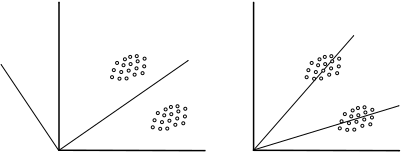
\includegraphics[width=0.75\textwidth]{nmf-svd.png}
\caption{\textbf{TODO redraw} Directions found by  SVD (on the left) vs directions by NMF (on the right)}
\label{fig:nmf-svd}
\end{figure}


The NMF of an $m \times n$ term-document matrix $D$ is $D \approx D_k = U  V^T$
where $U$ is an $m \times k$ matrix, $V$ is an $n \times k$ matrix and
$k$ is the number of semantic concepts in $D$.
Non-negativity of elements in $D_k$ is very good for interpretability: it
ensures that documents can be seen as a non-negative combination of
the key concepts.


Additionally, NMF is useful for clustering: the results of NMF can
be directly interpreted as cluster assignment and there is no need
to use separate clustering algorithms \cite{xu2003document}.

What is more, NMF is a co-clustering algorithms: it clusters both
rows of $D$ and columns of $D$ at the same time. For a term-document
matrix $D \approx U V^T$, where $U$ defines the reduced vector space for terms
and $V$ defines the reduced vector space for documents. Since all elements
are non-negative, it can have the following interpretation:
elements $(U)_{ij}$ of $U$ represent the degree to which terms $i$ belongs to cluster $j$,
and elements $(V)_{ij}$ represent the degree to which document $i$ belongs to cluster $j$.

\ \\

The document clustering using NMF consists of the following
steps \cite{xu2003document}:

\begin{itemize}
  \item Construct the term-document matrix $D$;
  \item Perform NMF on $D$ to get $U$ and $V$;
  \item Normalize rows $\mathbf v_i$ of $V$ by using $\mathbf v_i' = \mathbf v_i \cdot \| \mathbf u_i \|$ and rows $\mathbf u_i$ of $U$ with $\mathbf u_i' = \mathbf u_i / \| \mathbf u_i \|$;
  \item To determine the cluster assignment for document $\mathbf d_i$, examine $\mathbf v_i'$ (the $i$th row of $V$) and find the largest component of this vector. That is,
      $i$th document belongs to cluster $x$ if $x = \operatorname{arg \, max}_j v_{ij}$ where $v_{ij}$ are components of $\mathbf v_i$;
  \item If the desired number of clusters $K$ is larger than the rank $k$ of the reduced matrix $D_k$, the clustering can be performed directly on the rows of $V$, for example,
      by using $K$-Means.
\end{itemize}

% The computational complexity on NMF is $O(kn)$ 
